\documentclass[tikz,border=12pt]{standalone}
\usepackage[T1]{fontenc}
\usepackage{mathpazo}
\usepackage{amsmath,amssymb}
\usetikzlibrary{arrows.meta, positioning, calc, fit, decorations.pathreplacing}

\definecolor{stblue}{HTML}{7B97AD}
\definecolor{rwgold}{HTML}{B8995E}
\definecolor{sage}{HTML}{7A9A7E}
\definecolor{dkbrown}{HTML}{3D3530}
\definecolor{wmgray}{HTML}{7B7067}
\definecolor{cream}{HTML}{F9F6F0}
\definecolor{border}{HTML}{D4C9B8}
\definecolor{terracotta}{HTML}{C47A6A}
\definecolor{lavender}{HTML}{907EA0}

\begin{document}
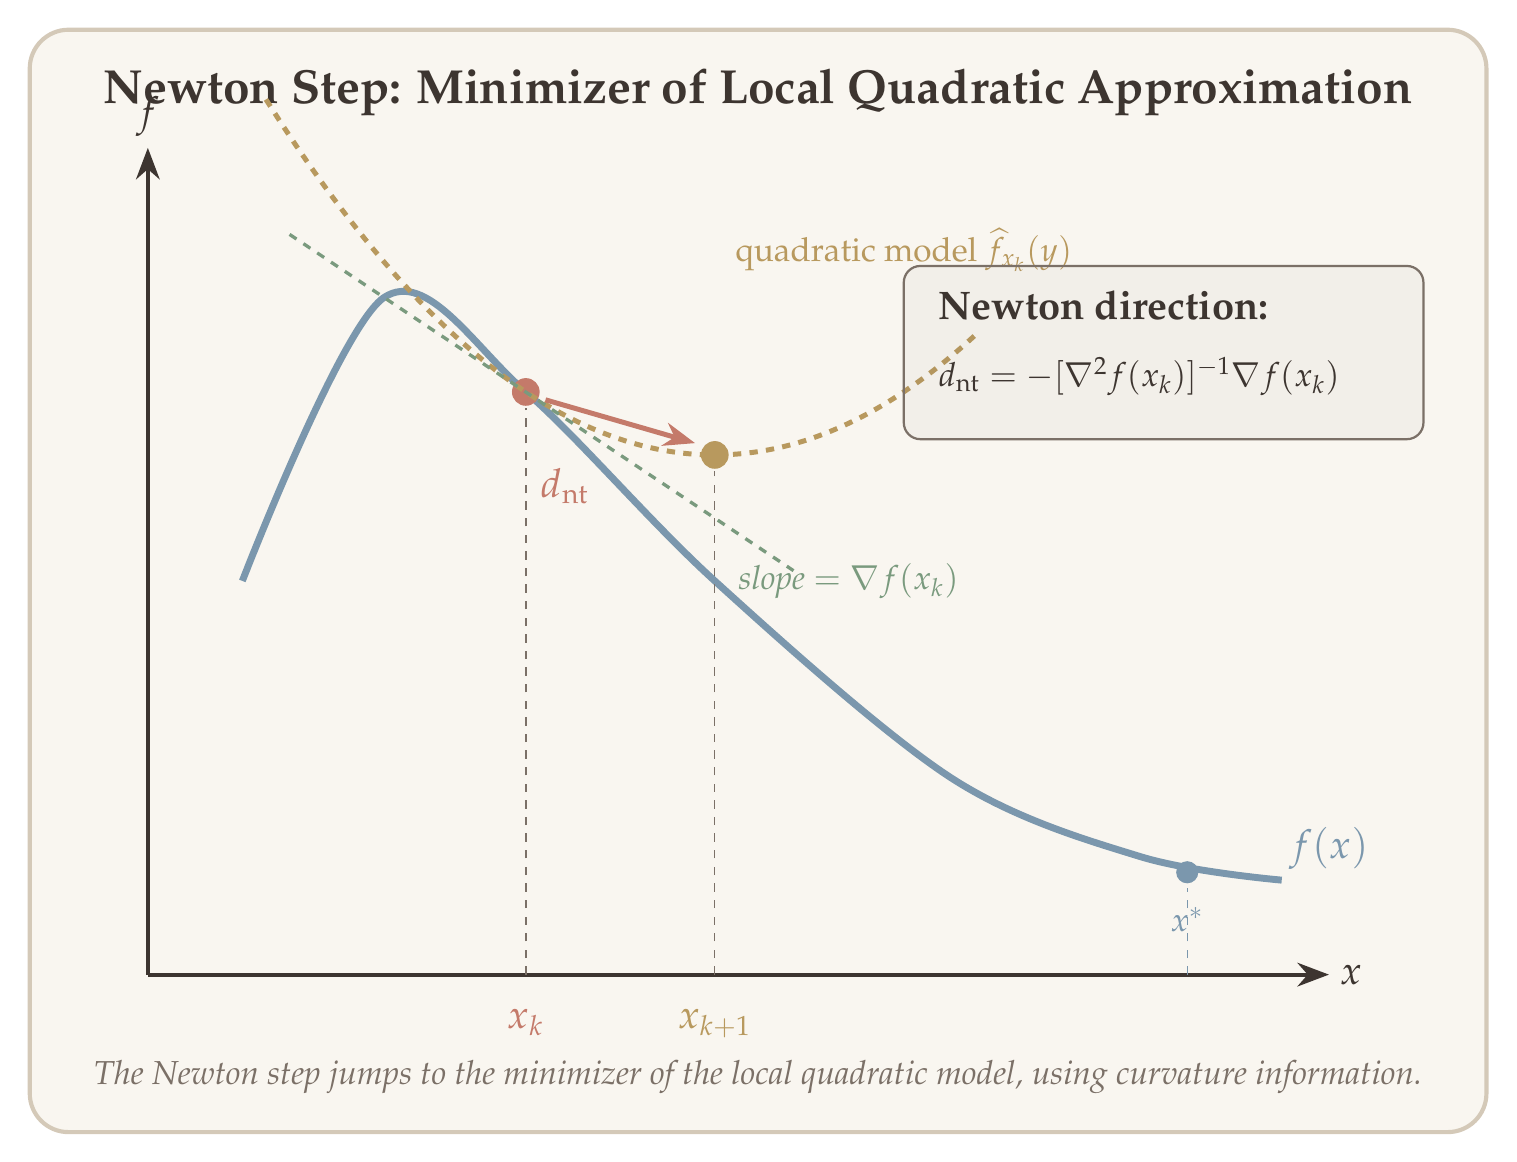
\begin{tikzpicture}[>={Stealth[length=4mm, width=3mm]}, line width=1.5pt]

% Background
\fill[cream, rounded corners=14pt] (-1.5,-2.0) rectangle (17,12);
\draw[border, line width=1.5pt, rounded corners=14pt] (-1.5,-2.0) rectangle (17,12);

% Title
\node[font=\LARGE\bfseries, text=dkbrown] at (7.75,11.2)
  {Newton Step: Minimizer of Local Quadratic Approximation};

% Axes
\draw[->, dkbrown, line width=1.5pt] (0,0) -- (15,0)
  node[right, font=\Large, text=dkbrown] {$x$};
\draw[->, dkbrown, line width=1.5pt] (0,0) -- (0,10.5)
  node[above, font=\Large, text=dkbrown] {$f$};

% True function f(x) -- smooth curve with minimum on the right
\draw[stblue, line width=2.5pt] plot[smooth, tension=0.55]
  coordinates {(1.2,5.0) (3.0,8.6) (4.8,7.4) (7.2,5.0) (10.2,2.5) (12.6,1.5) (14.4,1.2)};
\node[font=\Large\bfseries, text=stblue] at (15,1.6) {$f(x)$};

% Current point xk (on the curve at x=4.8, f=7.4)
\fill[terracotta] (4.8,7.4) circle (5pt);
\node[font=\Large\bfseries, text=terracotta, anchor=north] at (4.8,-0.3) {$x_k$};
\draw[wmgray, dashed, line width=0.5pt] (4.8,0) -- (4.8,7.2);

% Quadratic model tangent to f at xk
% f(xk)=7.4, slope=-0.667, curvature a=0.139
% f_hat(x) = 0.139*(x-4.8)^2 - 0.667*(x-4.8) + 7.4
% Minimizer at x=7.2, f_hat(7.2) = 6.6
\draw[rwgold, line width=1.8pt, dashed] plot[smooth, domain=1.5:10.5, samples=50]
  (\x, {0.139*(\x-4.8)*(\x-4.8) - 0.667*(\x-4.8) + 7.4});
\node[font=\large, text=rwgold] at (9.6,9.2) {quadratic model $\widehat{f}_{x_k}(y)$};

% Tangent line at xk (showing gradient direction)
\draw[sage, line width=1.2pt, dashed] (1.8,9.4) -- (8.2,5.13);
\node[font=\large\itshape, text=sage] at (8.9,5.0) {slope $= \nabla f(x_k)$};

% Newton step target: minimum of quadratic at x=7.2
\fill[rwgold] (7.2,6.6) circle (5pt);
\node[font=\Large\bfseries, text=rwgold, anchor=north] at (7.2,-0.3) {$x_{k+1}$};
\draw[wmgray, dashed, line width=0.5pt] (7.2,0) -- (7.2,6.4);

% Arrow from xk to xk+1 (Newton direction)
\draw[->, line width=1.8pt, terracotta] (5.05,7.3) -- (6.95,6.75);

% Newton step label
\node[font=\Large\bfseries, text=terracotta] at (5.3,6.2) {$d_{\mathrm{nt}}$};

% True minimizer x*
\fill[stblue] (13.2,1.3) circle (4pt);
\node[font=\large, text=stblue] at (13.2,0.7) {$x^*$};
\draw[stblue, dashed, line width=0.5pt] (13.2,0) -- (13.2,1.1);

% Annotation box
\draw[wmgray, line width=0.8pt, rounded corners=6pt] (9.6,6.8) rectangle (16.2,9.0);
\fill[wmgray, opacity=0.05, rounded corners=6pt] (9.6,6.8) rectangle (16.2,9.0);
\node[font=\Large\bfseries, text=dkbrown, anchor=west] at (9.9,8.5) {Newton direction:};
\node[font=\large, text=dkbrown, anchor=west] at (9.9,7.6) {$d_{\mathrm{nt}} = -[\nabla^2 f(x_k)]^{-1}\nabla f(x_k)$};

% Caption at bottom
\node[font=\large\itshape, text=wmgray] at (7.75,-1.3)
  {The Newton step jumps to the minimizer of the local quadratic model, using curvature information.};

\end{tikzpicture}
\end{document}
